\chapter{Controlling the dewetting morphologies of thin liquid films by switchable substrates}
\label{chapter:third_paper}
\epigraph{\textit{Du wirst nicht enttäuscht, wenn du nie etwas erwartest und bevor du etwas falsch machst, dann mach mal lieber gar nichts.}}{Kraftklub}

\textit{\small{This chapter has been submitted as a regular contribution to Physical Review Letters.}}\\

Switchable and adaptive substrates emerged as valuable tools for the control of wetting and actuation of droplet motion. Here we report a computational study of the dynamics of an unstable thin liquid film deposited on a switchable substrate, modelled with a space and time varying contact angle.
With a static pattern, all the fluid is drained into droplets located around contact angle minima, whereas for a sufficiently large rate of wettability variation a state consisting of metastable rivulets is observed. 
A criterion discriminating whether rivulets can be observed or not is identified in terms of a single dimensionless parameter.
Finally, we show and explain theoretically how the film rupture times, droplet shape and rivulet life time depend on the pattern wavelength and speed.
\\
\newcommand{\ts}{\textsuperscript}

\section{Introduction} Wet surfaces and droplets are part of our every-day experience and of numerous industrial processes including coating, tribology, painting and printing, to name but a few~\cite{gross1980fluid,szeri2010fluid,DERYCK1998278,doi:10.1146/annurev.fluid.31.1.347,dasilvasobrinhoStudyDefectsUltrathin1999,singh2010inkjet,jo2009evaluation,Wijshoff2010}. 
Moreover, the continuously growing technological interest for lab-on-a-chip devices~\cite{C6LC00387G,Focke} as well as for printable electronics~\cite{Kim_2005, Luechinger_2008} and printable photovoltaics~\cite{Brabec2001,RH20}, whose efficiency relies crucially on a precise control of material deposition upon (de-)wetting of liquid films, drew the attention to applications where the substrate is adaptive or switchable, i.e. it is not inert but responds dynamically to external stimuli or to the evolution of the coating liquid film itself~\cite{ButtEtAl_Langmuir2018,GuoGuo_RSCAdv2016}. 
Several realizations of switchable and adaptive substrates have been proposed~\cite{LiuChem2005, XiCSR2010}, involving smart materials such as polymer brushes~\cite{CohenStuartEtAl_NatMat2010,ayres2007stimuli,YongEtAl_Mat2018}, thermal-responsive hydrogels~\cite{ChenEtAl_SM2010}, light-responsive molecules and microstructures~\cite{ichimuraLightDrivenMotionLiquids2000,DelormeEtAl_Langmuir2005,OscuratoEtAl_AAMI2017} or processes such as electrowetting~\cite{MugeleEtAl_JPCM2005}.
Probably the simplest, yet non-trivial, modelling of a switchable substrate can be realized by a space and time dependent wettability pattern~\cite{D0SM02082F}. 
While a consistent body of theoretical/computational work has been devoted to processes on static heterogeneous substrates, though, the time dependent case is still almost unexplored, with few relevant exceptions focusing on single droplet spreading and sliding~\cite{D0SM02082F,GrawitterStark2,ThieleHartmann} or limited to an analysis of the linear regime~\cite{suman2006dynamics}.

In this Letter, we study, by means of numerical simulations, the full dewetting dynamics of a thin liquid film deposited over a substrate with a time varying wettability pattern, from rupture to the long time morphology. 
We identify two regimes where the rupture times grow with the pattern wavelength either linearly (on the static pattern) or attain a constant value (in the time dependent case), for short wavelengths, and approach a quadratic law as the wavelength increases. These observations are then explained theoretically.
We show that, by tuning the rate of change (the ``speed'') of the underlying pattern, it is possible to control, to some extent, the dewetting morphology. In particular, for large enough pattern speeds, we detect a metastable state, where the film retracts into metastable rivulets, eventually breaking up into multiple droplets.
We introduce a control parameter that discriminates whether rivulets or just droplets (as in the static situation)
can be observed and we propose a phenomenological argument that justifies the logarithmic dependence of the rivulets life time on the pattern speed.

\section{Method} In order to simulate the dewetting dynamics on patterned, ``switchable'', substrates, we integrate numerically the thin-film equation~\cite{reynoldsTheoryLubricationIts1886,oronLongscaleEvolutionThin1997,crasterDynamicsStabilityThin2009} 
\begin{equation}\label{eq:thinfilm}
    \partial_t h(\mathbf{x},t) = \nabla\cdot\left(M_{\delta}(h)\nabla p(\mathbf{x},t)\right),
\end{equation}
by means of a recently developed method, based on a lattice Boltzmann (LB) \\scheme~\cite{PhysRevE.100.033313,zitzLatticeBoltzmannSimulations2021, Zitz2022}.
Eq.~(\ref{eq:thinfilm}) describes, in a lubrication approximation spirit, the evolution of the height field (film thickness) $h(\mathbf{x},t)$, denoting the location of the liquid/air interface. The mobility function 
$M_{\delta}(h) = \frac{2h^3 + 6\,\delta\, h^2 + 3\delta^2h}{6\mu}$
depends on the velocity boundary condition at the substrate, parameterized by an effective slip length $\delta$
(for $\delta \rightarrow 0$ it reduces to the no-slip form $h^3/(3\mu)$). Here, $\mu$ is the fluid dynamic viscosity.
The film pressure $p(\mathbf{x},t)$ consists of the sum of the Laplace and disjoining pressures, that is $p(\mathbf{x},t) = -\gamma \nabla^2 h - \Pi$~\footnote{The Laplace pressure is the product of the surface tension 
and the local curvature, therefore its full expression reads $p_L = -\gamma \nabla^2 h/\sqrt{1+|\nabla h|^2}$; 
since we are in the lubrication regime, though, whereby $|\nabla h| \ll 1$, the denominator can be safely neglected 
and the pressure reduces to the form involving only the Laplacian of the thickness 
field~\cite{Benet2014,alizadeh_pahlavan_cueto-felgueroso_hosoi_mckinley_juanes_2018}.}, 
where $\gamma$ is the surface tension.
The disjoining pressure $\Pi$ can be seen as (minus) the derivative, with respect to the film thickness, of an effective interfacial potential.
As such, it contains the information on the liquid/solid and solid/gas interactions and, hence, on the wettability, which is parameterized in terms of the contact angle $\theta$~\cite{bonnWettingSpreading2009, schwartzSimulationDropletMotion1998}. 
The expression adopted for $\Pi$ is
\begin{equation}\label{eq:disjoinpressure}
\Pi(h,\theta) = \frac{2\gamma}{h_{\ast}}(1-\cos(\theta(\mathbf{x},t)))
  f\left(\frac{h}{h_{\ast}}\right),
\end{equation}
where $f(\xi)=\xi^{-3} - \xi^{-2}$ and $h_{\ast}$ is the height at which the disjoining pressure vanishes and sets the precursor layer thickness~\footnote{Expressions of 
the general form $\Pi(h) = \gamma(1-\cos \theta)(n-1)(m-1)/(n-m)((h_{\ast}/h)^n - (h_{\ast}/h)^m)/h_{\ast}$
are frequently found in the literature, with various combination of exponents $(n,m)$ ($n>m$), depending
on the type of interactions among fluid molecules and between fluid and substrate~\cite{schwartzSimulationDropletMotion1998,Mitlin,Teletzke}. A common choice, for instance, is the pair $(9,3)$, which 
can be derived from molecular interactions of Lennard-Jones type. Here, the use of the $(3,2)$ pair is motivated mainly by the computational advantage of keeping the characteristic dewetting time 
shorter. We have run also a single case ($\lambda=256 h_0$ and $\Gamma=1.5$) with $(9,3)$ and observed that 
the dynamics remains essentially the same, but for a shift in the time scale (see also~\cite{zitzLatticeBoltzmannSimulations2021})}.
The time variation of the patterned substrate then enters the model precisely through the disjoining pressure, by making the contact angle space and time dependent, i.e. $\theta = \theta(\mathbf{x},t)$.
We decorate the substrate with a checkerboard pattern, a common choice that generalizes the broken homogeneity of the stripes to two 
directions~\cite{KarguptaLangmuir2003,Jalali2018,Nagayama2020,Das2020}.
In particular, we employ the sinusoidal form
\begin{equation}\label{eq:sinetheta}
   \!\! \theta(\mathbf{x},t) = \theta_0 + \delta\theta\left[\sin\left(q_{\theta} (x+v_{\theta x}t)\right)\sin\left(q_{\theta}(y+v_{\theta y}t)\right)\right],\! 
\end{equation}
where $q_{\theta} = 2\pi/\lambda$, i.e.~the pattern evolves in time as a plane wave.
A possible laboratory experiment for the here mentioned approach consists of a light switchable substrate with a thin film cast on it~\cite{beckerComplexDewettingScenarios2003, IchimuraEtAl_Science2000}. 
The external stimulus, our moving pattern, can be realized, e.g., by using a digital multimirror device (DMD)~\cite{doi:10.1021/jp301092y,doi:10.1126/science.aax8760}.
We fix the velocity direction to one diagonal, namely $\mathbf{v}_{\theta} = (v_{\theta x},v_{\theta y}) = v_{\theta}(1/\sqrt{2},-1/\sqrt{2})$ (we will return later on the importance of this choice), and we set $\theta_0 = 20^{\circ}$ and $\delta\theta=10^{\circ}$~\footnote{Notice that, since a typical velocity is such that $v_{\theta} \Delta t \ll \Delta x$ (in one LB time step $\Delta t$ the wave would travel a distance much smaller than a lattice spacing $\Delta x$),
the time update needs to be interpreted in an integer part sense, that is the pattern is shifted by one $\Delta x$ every $1/v_{\theta x}$ time steps (and equivalently in the $y$-direction).}.
Lengths and time scales will be expressed, respectively, in units of the mean film height, $h_0$ (which is constant in time, due to mass conservation), and of $t_0 = \frac{3\mu}{\gamma h_0^3 q_0^4}$, the inverse growth rate of the most unstable mode, whose wavenumber is $q_0$, of a spinodally dewetting film \cite{meckeThermalFluctuationsThin2005}. On a uniform substrate, with constant contact angle $\theta^{(u)}$, the wavenumber reads 
$(q^{(u)}_0)^2 = h_{\ast}^{-2}(1-\cos \theta^{(u)})f^{\prime}(h_0/h_{\ast})$ \cite{meckeThermalFluctuationsThin2005,zhangMolecularSimulationThin2019}. In our patterned case, we define 
  $q_0^2=h_{\ast}^{-2}(1-\cos\theta_0)f^{\prime}(h_0/h_{\ast})$. Correspondingly, we choose as a velocity scale $v_0 = \lambda_s/t_0$, where
$\lambda_s = 2\pi/q_0$.
\begin{figure}
    \centering
    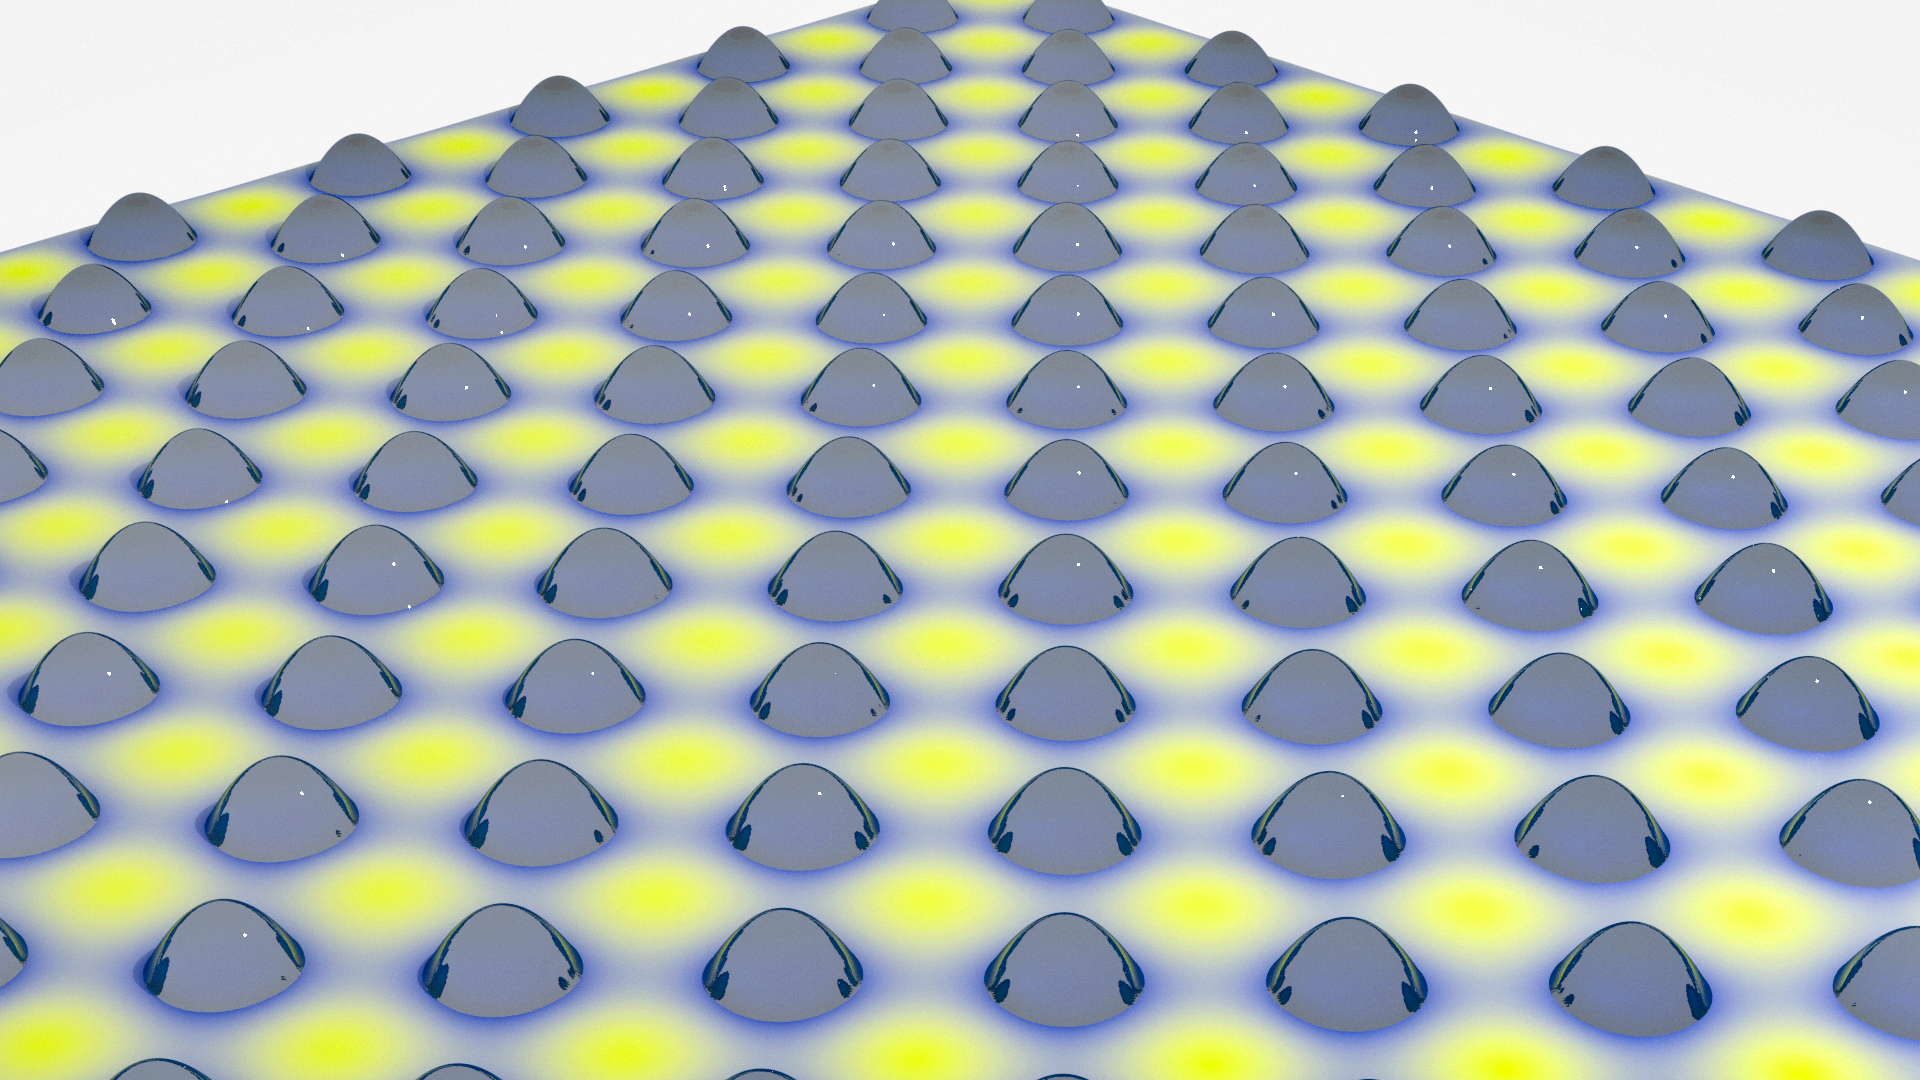
\includegraphics[width=0.75\textwidth]{graphics/Figure_1.png}
    \caption{Stationary film thickness field ($t>t_0$) showing the formation of droplets. The color map indicates the contact angle pattern 
    (Eq.~(\ref{eq:sinetheta}) with $v_{\theta}=0$), with lower (higher) values coded in light blue (yellow).
    }
    \label{fig:handtheta}
\end{figure}
%%%%
To give a flavour of how to compare with actual experimental systems, let us notice
first that the expression of $t_0$ depends on the disjoining pressure (through its dependence 
 $q_0 = \sqrt{\frac{1}{2\gamma} \Pi^{\prime}(h_0)}$) and contains, therefore, energetic details, namely 
 the Hamaker constant $A_H$. Consider, for instance, the problem studied in \cite{beckerComplexDewettingScenarios2003}: the dewetting of a polystyrene film of thickness $h_0 \approx 4 \, \text{nm}$ deposited on a silicon 
dioxide substrate, where $A_H  = 2.2 \times 10^{-20} \, \text{J}$ and 
$\gamma = 0.03 \, \text{N}/\text{m}$. Neglecting the short range part of the interface potential
(such that $\Pi(h)= - \frac{A_H}{6\pi h^3}$)~\cite{meckeThermalFluctuationsThin2005,beckerComplexDewettingScenarios2003}, one gets 
$q_0^2 \approx \frac{A_H}{4\pi \gamma h_0^4} \approx 2.5 \times 10^{-4} \, \text{nm}^{-2}$.
The characteristic time of the growth of the instability for these experiments, then, reads \cite{fetzerThermalNoiseInfluences2007} (the dynamic viscosity of polystyrene is 
$\mu = 1.2 \times 10^4 \, \text{Pa} \cdot \text{s}$) $t_0 = \frac{3\mu}{\gamma h_0^3 q_0^4} \approx 300 \, \text{s}$ and it can be seen that indeed film rupture occurs within time 
scales of the order of $t_0$ ($\approx 2 t_0$) \cite{beckerComplexDewettingScenarios2003}, as in our 
simulation for the largest pattern wavelength, $\lambda = L$ (see also our previous work
with homogeneous substrates~\cite{zitzLatticeBoltzmannSimulations2021}).
%%%%
All our simulations are run on a bi-periodic square domain of size $L \times L$ with 
$L/h_0 = 512 $. The numerical values in lattice Boltzmann units of the 
mean film thickness, dynamics viscosity and surface tension are, respectively, $h_0=1$, $\mu=1/6$
and $\gamma=0.01$.
To regularize the contact line divergence~\cite{huh1971hydrodynamic} we use a precursor layer thickness $h_{\ast}/h_0=0.07$ and a slip length $\delta/h_0 = 1$, 
a value which lies
within the weak/intermediate slip regime~\cite{peschkaSignaturesSlipDewetting2019,fetzer2007quantifying, munchLubricationModelsSmall2005} (we have tried also a value four times smaller, without observing 
any major qualitative change in the results).
The liquid film is initialized with a height field slightly perturbed around the mean value $h_0$, i.e. $h(\mathbf{x},0) = h_0 \left[1 + 0.1 \left(\sin\left(\frac{2\pi x}{L}\right)\sin\left(\frac{2\pi y}{L}\right)\right)\right]$.
Various wavelengths, in the range $\lambda/h_0 \in [64, 512]$, and velocities,
$v_{\theta}/v_0 \in [0, 200]$, are considered for the wettability pattern, Eq.~(\ref{eq:sinetheta}). 
A few comments on these ranges are noteworthy at this point. The wavelengths are obviously limited from above by the size of the computational domain. On the other extreme, too short wavelengths are prevented by
the energetic cost of accomodating droplets on too
small patches, since the local contact angle 
(that increases with decreasing $\lambda$~\cite{SuppMat}) would possibly exceed the largest substrate contact angle, such that the patterning 
itself would loose meaning. 
It has been, in fact, proven, both theoretically and experimentally, that 
for the confinement to be effective, the pattern characteristic size should 
not be much smaller than the spinodal length scale on the less wettable substrate
\cite{KarguptaJCP2002,KarguptaLangmuir2000,Nisato1999,Karim1998}.
We keep, therefore, $\lambda \stackrel{>}{\sim} \lambda_s \approx 70 h_0$.
The pattern speeds, on the other hand, are limited by the intrinsic LB bound of the lattice speed of sound
 \cite{succi}.\\
The Reynolds number, $Re$, is of the order of $Re \sim 10^{-2}$ on the 
static substrate and never exceeds the value $\approx 0.2$ in the time dependent case.
In Fig.~\ref{fig:handtheta} we show $h(\mathbf{x},t)$ (droplets) and $\theta(\mathbf{x})$ (color coded) for $v_{\theta} = 0$ (i.e. the static case) and $\lambda = 256 h_0$\footnote{For a better visualization we take twice the domain length $L$ and periodically continue the image.}, in late stages of dewetting.
As expected, droplets form in regions of small contact angles (blue) while the regions of high contact angles (yellow) dewet.

\section{Results} We start our analysis studying, first, how the rupture times depend on the parameters characterising the wettability pattern, namely the wavelength of the contact angle variation, $\lambda$, and wave speed, $v_{\theta}$.
The film rupture time, $\tau_r$, is defined as the least $t$ such that $h(\mathbf{x},\tau_r)=h_{\ast}$ (that is, when the free surface "touches" the substrate).
In Fig.~\ref{fig:model_rt} we report the rupture times, as a function of the wavelength, for stationary ($v_{\theta}=0$) and time-dependent ($v_{\theta}=20 v_0$) patterns. 
It is conveyed that, overall, rupture occurs earlier on the static substrate, suggesting that the time variation tends to stabilize the film, in agreement with linear stability analysis results~\cite{suman2006dynamics}.
We observe that $\tau_r$ grows linearly with $\lambda$, for short wavelengths, and quadratically for longer $\lambda$.
These facts can be explained, qualitatively, as follows. 
Let us first notice that the film rupture consists of two processes, each with its associated time scale: the growth of unstable interface perturbation with rate $t_{\theta}^{-1}$, and the retraction of liquid from more hydrophobic regions, occurring in a characteristic time $t_R$. For longer pattern wavelengths, the dewetting instability amplifies more slowly, such that it is reasonable to take it as the process determining the rupture time, $\tau_r \sim t_{\theta}$.
In this case, from the linearized thin-film equation (in one spatial dimension, for simplicity), obtained setting $h=h_0 + \delta h$ with $\delta h \ll h_0$, 
we can easily see that the exponential growth of the height perturbation is affected by the wettability pattern (variable contact angle) in such a way that $\partial_t (\delta h) \propto (\partial_x^2 (\partial_h\Pi(h_0))) \delta h$. Therefore, since the characteristic time $t_{\theta}$ can be estimated dimensionally as $t_{\theta} \sim \delta h/\dot{(\delta h)}$, the rupture time should go as
\begin{multline}\label{eq:taur_l2}
    \tau_r \sim t_{\theta} \sim  \delta h/\dot{(\delta h)} \propto \frac{3\mu}{h_0^3}(\partial_x^2 (\partial_h\Pi (h_0)))^{-1} \sim t_0 \left(\frac{q_{\theta}}{q_0}\right)^{-2} \propto t_0 q_0^2 \lambda^2.
\end{multline}
Conversely, for fast growths ($t_{\theta} \ll t_R$), retraction dominates and fixes the time scale, $\tau_r \sim t_R$. 
The latter is related to the time the liquid takes to flow out of regions of high contact angle, whose size is $\sim \lambda$. Hence we have 
\begin{equation}\label{eq:taur_l1}
 \tau_r \sim \tau_R \propto \frac{1}{U_{\Theta}}\lambda,
\end{equation}
where $U_{\Theta}$ is the retraction speed $U_{\Theta} = \frac{\gamma \Theta^3}{9\mu}$~\cite{edwardsNotSpreadingReverse2016}, with $\Theta = \max_{\mathbf{x}}\theta(\mathbf{x})$.
\begin{figure}
    \centering
    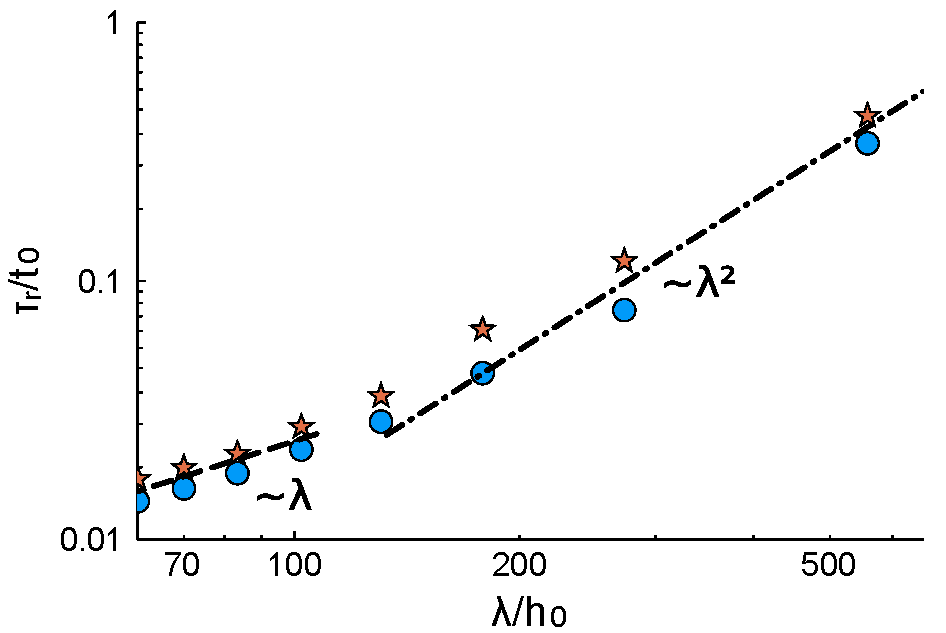
\includegraphics[width=0.75\textwidth]{graphics/Figure_2.pdf}
    \caption{Rupture times, $\tau_r$, as a function of the pattern wavelength $\lambda$, for $v_{\theta}=0$ (\textcolor{jlblue}{$\bullet$}) and $v_{\theta}=20 v_0$ 
    (\textcolor{jlorange}{$\star$}).
    The continuous and dashed lines indicate the linear, $\sim \lambda$, and quadratic, $\sim \lambda^2$, scaling laws, respectively.
        }
    \label{fig:model_rt}
\end{figure}
We now focus on the long time dynamics and in particular on the characterization of the dewetting morphologies and how they are affected by the speed of the wettability wave.
\begin{figure}
    \centering
    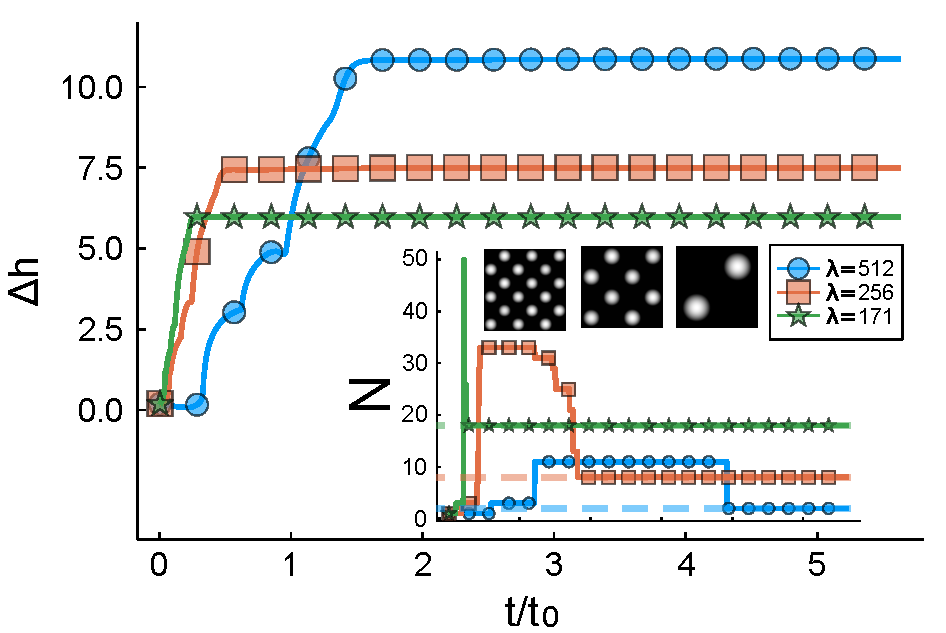
\includegraphics[width=0.75\textwidth]{graphics/Figure_3.pdf}
    \caption{MAIN PANEL: Time evolution of the height fluctuations, $\Delta h(t)$, during the dewetting process on the patterned substrate given by       
    Eq.~(\ref{eq:sinetheta})
    with $v_{\theta}= 0$ and $\lambda= 512 h_0$ (blue circles), $\lambda=256 h_0$ (orange squares) and $\lambda=170 h_0$ (green stars).
    The dashed lines indicate the geometrically expected values of the droplet height $h_d$, assuming monodispersity and a perfect spherical cap shape. 
    INSET: Number of droplets, $N(t)$, as a function of time. The three horizontal dashed lines indicate the number of minima of Eq.~(\ref{eq:sinetheta}),
      which is $2\left(\frac{L}{\lambda}\right)^2$. In the insets, we display snapshots of the stationary droplet states as grey-scale images
      of the film thickness field, $h(\mathbf{x},t)$.
      }
    \label{fig:clusters_v0_sine}
\end{figure}
On the stationary substrate, after rupture all the fluid accumulates in droplets centered at contact angle minima.
Consequently, as we see from the inset of Fig.~\ref{fig:clusters_v0_sine}, where we plot the number of droplets $N(t)$ in time\footnote{A droplet is identified by the set (``cluster'') of points, in the plane, constituting each of the connected components of the set $\{\mathbf{x} \in [0,L]^2 | h(\mathbf{x},t) \geq h_{\ast}$\}; the clusters are determined by means of an algorithm of Hoshen-Kopelman type~\cite{HK}.}, in the steady state ($t \gg t_0$) $N(t)$ attains the value $N_{\infty} = 2(L/\lambda)^2$ (reported as horizontal lines), which equals the minima of Eq.~(\ref{eq:sinetheta}), for $v_{\theta}=0$.
Notice that the number of droplets converges faster for smaller pattern wavelengths, in line with the observation reported and justified in the previous section that the characteristic dewetting time decreases with the wavelength.\\
In the main panel of the same figure, we see that the height fluctuations $\Delta h(t) = \max_{\mathbf{x}}\{h(\mathbf{x},t)\}-\min_{\mathbf{x}}\{h(\mathbf{x},t)\}$
grow in time until film rupture and then settle to a constant value, which represents a measure of the mean droplet height $h_d$ (since
droplets are essentially monodisperse), decreasing with the pattern wavelength (as expectable, due to the decrease of the droplet volume,
$V_d = \frac{h_0 \lambda^2}{2}$).\\
\begin{figure}
    \centering
    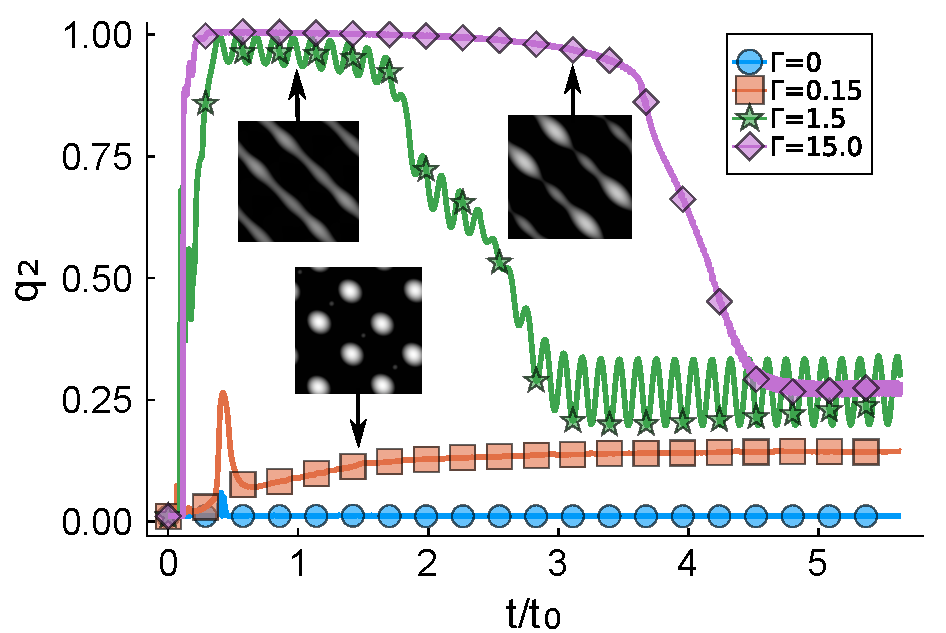
\includegraphics[width=0.75\textwidth]{graphics/Figure_4.pdf}
    \caption{Time evolution of the second order Minkowski structure metric, $q_2(t)$ (see text for details), for different $\Gamma$ values, on a substrate with pattern wavelength $\lambda=256 h_0$.
    The grey-scale insets supply snapshots of the film thickness field associated to the various curves.
    }
    \label{fig:msm_q2}
\end{figure}
A time-dependent pattern affects the dewetting morphology quite substantially.
For $v_{\theta} = 0.2 v_0$ we still observe the formation of droplets, similarly to the stationary case ($v_{\theta} = 0$). However, these are transported with the contact angle minima, reproducing a somehow similar behaviour recently described in a numerical study of a droplet on a moving wettability step~\cite{D0SM02082F}.
If the pattern speed is further increased, for $v_{\theta} = 2 v_0$ we observe the development of rivulet-like structures, aligned with $\mathbf{v}_{\theta}$. 
The film, in fact, while dewetting in the direction normal to the pattern velocity, is exposed, in the direction of the velocity, to a periodic potential with alternating minima and saddle points, which partially (as we will see) stabilizes the film over ``preferential'' lanes along the diagonals. 
This makes the chosen velocity direction, $(1/\sqrt{2},-1/\sqrt{2})$ (or, equivalently, the orthogonal one $(1/\sqrt{2},1/\sqrt{2})$), optimal for the formation of rivulets. 

In order to better characterize the various morphologies we apply the theory of Minkowski's functionals. 
In particular, we employ the second order Minkowski structure metric, $q_2$~\cite{doi:10.1063/1.4774084, Schaller2020}, which can be computed from a Voronoi tessellation of the set of discrete points $(x_i, y_i)$ on the 2D lattice, such that the height field lies above a certain threshold\footnote{The expression is: $q_2 = \frac{1}{N}\sum_j \frac{1}{P_j}|\sum_k L^{(j)}_k e^{2i\phi^{(j)}_k}|$, where the inner sum runs over the edges of length $L^{(j)}_k$, of the $j$-th Voronoi cell, whose perimeter is $P_j$, and $\phi^{(j)}_k$ is the polar angle of the normal to the $k$-th edge. 
The outer sum represents an ensemble average over the $N$ points in the set.}. The $q_2$ metric quantifies the degree of anisotropy of the dewetting morphology, so it takes relatively large values if the structures formed display a preferential direction. 
Measuring $q_2$ then enables us to clearly distinguish between the formation of droplets and rivulets: much larger $q_2$ values are attained for the latter type of structure, as we can see in Fig.~\ref{fig:msm_q2}.
We observe, on the other hand, that such rivulets are metastable and eventually break up into droplets, as indicated by the collapse of $q_2$ at later times. 
Notice, though, that the $q_2$ signal for any $v_{\theta} >0$ always stays above the one for the static case, suggesting that even the smallest pattern velocity introduces a sizeable deformation of the spherical cap shape.
\begin{figure}
    \centering
    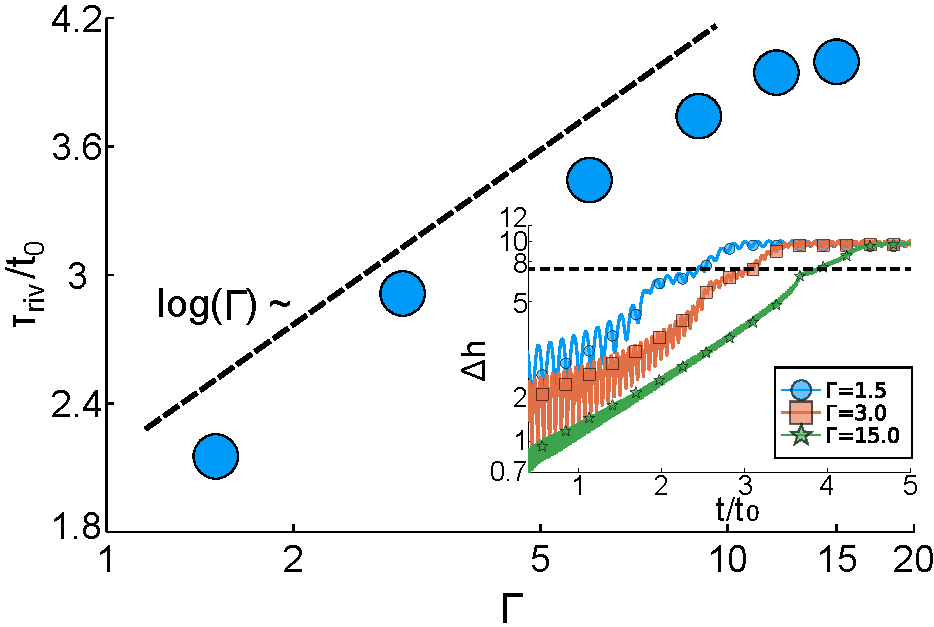
\includegraphics[width=0.75\textwidth]{graphics/Figure_5.pdf}
    \caption{MAIN PANEL: Rivulets life-times, $\tau_{\text{riv}}$, for various $\Gamma$ values.
    The dashed line is plotted as a guide to the eye to highlight the logarithmic dependence, in agreement with 
    the theoretical prediction, Eq.~(\ref{eq:rivlt}).
    INSET: Height fluctuations, $\Delta h(t)$, vs time, computed along the rivulet axis, for three different $\Gamma$ values.
    }
    \label{fig:stab_ligs_lam2}
\end{figure}
The breakup is the result of a varicose mode of the rivulet~\cite{doi:10.1063/1.3211248, PhysRevE.77.061605}, whose wavelength is $\approx\lambda$, such that only $N_{\infty}/2$ droplets are counted after breakup. 
These droplets show a peculiar dynamics, characterized by a periodic sequence of spreading and retraction, driven by the pattern, that we dub "pumping state"~\footnote{see movie file ligament\_formation\_and\_breakup.mp4 in~\cite{SuppMat}.}.

We argue that the emergence of rivulets is controlled by the competition of two characteristic velocities: the pattern wave speed, $v_{\theta}$, and the retraction speed, $U_{\Theta}$, introduced in Eq.~(\ref{eq:taur_l1}). 
If $U_{\Theta}$ is large as compared to $v_{\theta}$, the film retraction is faster than the transport due to the contact angle field and thus droplets from. However, if $v_{\theta}$ is larger than $U_{\Theta}$, then the retracting film has too little time to form droplets and ends up in the metastable rivulet state. It appears, therefore, natural to consider the ratio of these two velocities, 
$\Gamma \equiv v_{\theta}/U_{\theta}$, as the discriminating parameter.
We see from Fig.~\ref{fig:msm_q2} that indeed rivulets form only for $\Gamma > 1$. 
Moreover, the larger $\Gamma$, the more stable the rivulets are; in other words, the rivulet life-time, $\tau_{\text{riv}}$, that can be conventionally taken as the time at which the drop of $q_2$ occurs, grows with $v_{\theta}$ (see Fig.~\ref{fig:stab_ligs_lam2}).
The rivulet itself is, in fact, prone to dewetting, with the liquid accumulating over patches around contact angle minima. However, as the pattern moves, the instability is tamed due to configurations whereby higher contact angle regions underlie height field maxima, thus tending to revert the fluid flow.
Heuristically speaking, this means that, if we evaluate $\Delta h(t)$ restricted on the rivulet axis, this should grow exponentially (with a certain growth rate $\alpha \propto t_0$) only when the system is in the unstable configuration. Namely, $\Delta h(t)/\Delta h_0 \propto e^{\alpha t}$ (see inset of Fig.~\ref{fig:stab_ligs_lam2}) with a prefactor proportional to the time spent by the rivulet in such a configuration, which goes as $\sim \lambda/v_{\theta}$, therefore 
$\Delta h(t)/\Delta h_0 \sim \alpha (\lambda/v_{\theta})e^{\alpha t}$. 
The rivulet life-time can be seen as the rupture time of the structure along its axis, hence such that $\Delta h (\tau_{\text{riv}}) \sim h_0$ \cite{zitzLatticeBoltzmannSimulations2021}, which yields
\begin{equation}\label{eq:rivlt}
    \tau_{\text{riv}} \sim \alpha \log(v_{\theta}) \propto t_0 \log(\Gamma). 
\end{equation}
This logarithmic dependence is indeed observed in the numerical data as shown in Fig.~\ref{fig:stab_ligs_lam2}.\\
Before concluding, we would like to envisage a possible realization of a 
dewetting experiment on a switchable substrate of the type modelled by the spatio-temporal 
contact angle (\ref{eq:sinetheta}). One may think of a thin liquid film cast on a light responsive substrate~\cite{IchimuraEtAl_Science2000}, under the action of controlled 
external stimuli (a light emitter). 
An ideal candidate could be a digital multimirror device (DMD).
This technology has effectively been used for thin film experiments and additive manufacturing~\cite{doi:10.1021/jp301092y, doi:10.1126/science.aax8760}, it allows for fast temporal modulations of the optical signal (with frequencies up to $\approx 16 \, \text{kHz}$)
with spatial resolution of $\approx 10 \times 10 \, \mu \text{m}^2$ (the size of a pixel).
Considering as a reference, for instance, the system studied in ~\cite{beckerComplexDewettingScenarios2003,fetzerThermalNoiseInfluences2007}, namely a $\sim 4 \, \text{nm}$ thick film 
of polystyrene deposited on an oxidized silicon wafer,  
we evaluate the retraction speed 
$U_{\Theta} = \frac{\Theta^3 \gamma}{9 \mu}$ to be 
$U_{\Theta} \approx 10^{-2} \, \mu \text{m}/\text{s}$. 
The (minimum) \textit{pattern speed} can be 
estimated, from the pixel size with frame rate $\sim 1 s^{-1}$, as 
$v_{\theta} \sim 10 \, \mu \text{m}/\text{s}$, that would give $\Gamma \sim 10^3$, i.e. well within the rivulet regime ($\Gamma > 1$). We note, also, that both $U_{\Theta}$ and $v_{\theta}$ can be widely modulated: the former, playing either with the (temperature and molecular weight dependent) viscosity 
or tailoring the substrate to making it more hydrophobic (i.e. increasing the contact angle); the latter, tuning
the spatial resolution and frame rate of the DMD. We expect, thus, the range of achievable $\Gamma$'s to 
be feasibly extended both to very high ($\Gamma \gg 1$) and very low ($\Gamma \ll 1$) values.\\

\section{Conclusions}
We have presented results, from numerical simulations and theoretical analysis, on the dewetting of thin liquid films on a switchable substrate, modelled with a space and time periodically varying contact angle in the thin-film equation.
Studying how the stability of the film depends on the underlying static pattern, we found that the rupture times grow linearly with the pattern wavelength, for short wavelengths, and quadratically in the long wavelength limit. 
In the time-dependent case, the rupture times are in general longer, indicating an induced greater film stability, and, while the quadratic growth is preserved at long wavelengths, a plateauing behaviour is observed as the wavelength decreases. 
A theoretical explanation has been provided for all these various regimes.
Furthermore, we showed that, at increasing the wettability wave speed, a transition occurs in the dewetting morphology from a multi-droplet to a metastable multi-rivulet state. 
A dimensionless parameter, $\Gamma$, controlling the transition has been identified in the ratio of the pattern speed and the typical film retraction speed over the substrate. 
The rivulets life-time itself grows with the pattern speed, displaying a logarithmic dependence that has been captured by means of phenomenological arguments.
On a broader perspective, our work suggests that switchable substrates offer a new avenue to control thin film dewetting, with obviously relevant implications, for instance, for open microfluidic devices, and paves the way to future studies in this direction, exploiting more complex and dedicated space-time dependencies.

\section{Acknowledgements} SZ and JH acknowledge financial support from the Deutsche Forschungsgemeinschaft (DFG) within the priority program SPP2171 ``Dynamic Wetting of Flexible, Adaptive, and Switchable Substrates'', project HA-4382/11.
\newpage
\section{Supplemental Material}.
\subsection{Minkowski's structure metric \texorpdfstring{$q_2$}{hmm} in an extended parameter space.}
\begin{figure}
    \centering
    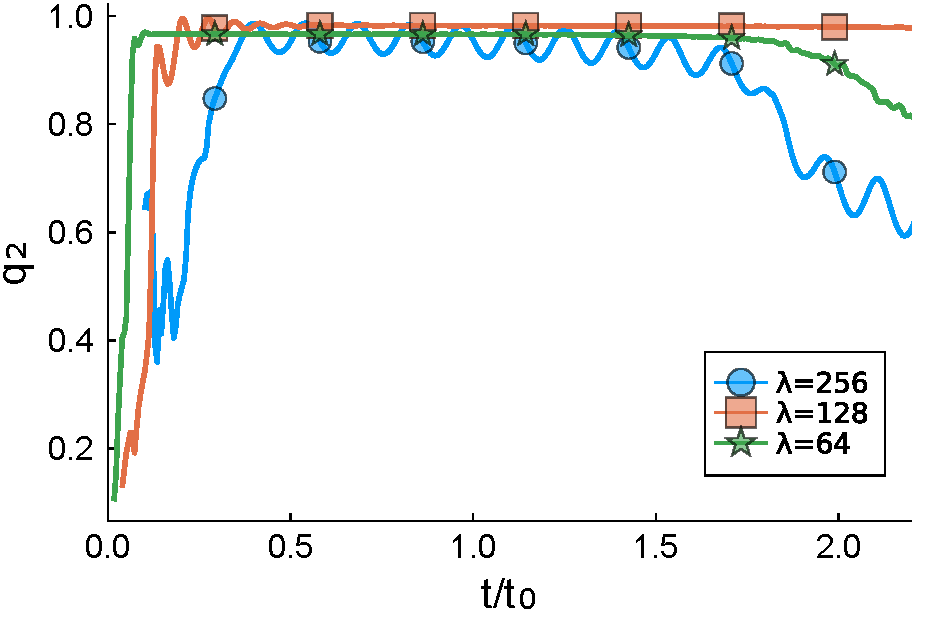
\includegraphics[width=0.4\textwidth]{graphics/SupMatFig_1.pdf}
    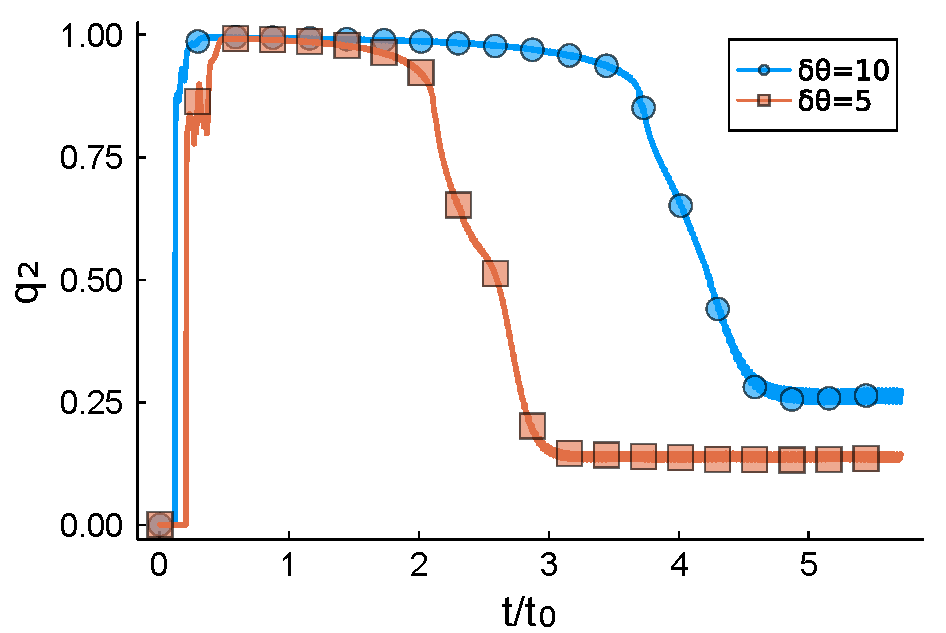
\includegraphics[width=0.4\textwidth]{graphics/SupMatFig_2.pdf}
    \caption{LEFT PANEL. Minkowski's structure metric $q_2$ for three different wavelengths $\lambda=64 h_0$, $\lambda=128 h_0$ and 
    $\lambda=256 h_0$ (as in figure 4 of the main text) and for $\Gamma=1.5$ (all other parameters are as in the main text). 
    The time interval during which $q_2 \approx 1$ signals the emergence of rivulets, also for $\lambda = 64 h_0$ which is comparable with the spinodal wavelength $\lambda_s \approx 70 h_0$. RIGHT PANEL. Comparison of the Minkowski's structure metric $q_2$ for $\delta\theta=5^{\circ}$ and $\delta\theta=10^{\circ}$, 
    $\Gamma = 15$ and $\lambda = 256 h_0$.}
    \label{fig:q2_difflambda}
\end{figure}
\noindent In this section we test the robustness of the observation of the rivulet 
state over a wider parameter space and in particular at changing: 1) the 
pattern wavelength $\lambda$ and 2) the heterogeneity amplitude $\delta \theta$.
To this aim we have run simulations with $\Gamma=1.5$, $\lambda/h_0 = 64, 128$, and with $\Gamma = 15$, $\lambda = 256 h_0$, $\delta \theta = 5^{\circ}$, respectively.
In Fig.~\ref{fig:q2_difflambda} (left panel) we report the measurements of the Minkowski's structure metric $q_2$, whose 
increase from zero up to a plateauing value of $q_2 \approx 1$ indicates the emergence of rivulets, for 
the different $\lambda$'s ($\lambda=256 h_0$, which is the value considered in the main text, is also reported 
for comparison).
Analogously, in the right panel, we report $q_2$ as a function of time for  
$\delta \theta = 5^{\circ}$  and $\delta \theta = 10^{\circ}$ (the value used in the main text). 
We see that the $q_2$ metric attains the value $q_2 \approx 1$, signalling the rivulet state, albeit over 
a time interval shorter than for $\delta \theta = 10^{\circ}$, i.e. the rivulets lifetime decreases with 
$\delta \theta$. This was somehow expected, since obviously (and also in the static case) 
the patterning looses effectiveness as the contact angle mismatch is reduced (see, e.g.~\cite{PhysRevLett.84.931}).

\subsection{Droplet shape}

\noindent We investigate, here, how the local contact angle of droplets, formed on the more
hydrophilic patches after dewetting, depends on the pattern wavelength. We recall, in fact,
that the patterning is such that the contact angle is not piecewise constant, but varies
with continuity.
The droplet shape is determined by minimization of the total interfacial energy
\begin{equation}\label{eq:energy}
E = \gamma_{\text{lg}} A_{\text{lg}} + \int_{A_{\text{sl}}} (\gamma_{\text{sl}} - \gamma_{\text{sg}})d \sigma,
\end{equation}
where $A_{\text{lg}}$ and $A_{\text{sl}}$ are the liquid/gas and solid/liquid interface areas, and $\gamma_{\text{lg}}$, $\gamma_{\text{sl}}$,
$\gamma_{\text{sg}}$ are the liquid/gas, solid/liquid and solid/gas interface energies 
per unit area \cite{D0SM00196A}. 
In particular, $\gamma_{\text{lg}} \equiv \gamma$ is the surface tension.
Setting $A_{\text{lg}} \equiv A$ and $A_{\text{sl}} \equiv S$, by Young's equation 
$\cos \theta = \frac{\gamma_{\text{sg}} - \gamma_{\text{sl}}}{\gamma}$,
Eq.~(\ref{eq:energy}) can be rewritten as
\begin{equation}\label{eq:energyoung}
\tilde{E} \equiv \frac{E}{\gamma} = A - \int_S \cos \theta \text{d}x \text{d}y.
\end{equation}
Droplets will form around minima of the contact angle pattern
\begin{equation}\label{eq:contact}
\theta(x,y) = \theta_0 + \delta \theta \sin(q_{\theta} x) \sin (q_{\theta} y) \qquad q_{\theta} = \frac{2\pi}{\lambda},
\end{equation}
namely $(x_n,y_n) = \left((2n+1)\frac{\lambda}{4},(2n+3)\frac{\lambda}{4}\right)$, with
$n=0,\pm 1, \pm 2,\dots$.
If we consider large wavelengths ($q_{\theta} h_0 \ll 1$) and heterogeneity
($\delta \theta \ll 1$) such that the contact angle gradients are small, the
expression (\ref{eq:contact}) can be expanded as
\begin{equation}\label{eq:contact2}
\theta(x,y) \approx \theta_m + \delta \theta q_{\theta}^2 ((x-x_n)^2 + (y - y_n)^2) + o(|\mathbf{x}-\mathbf{x}_n|^2),
\end{equation}
where $\theta_m = \theta_0 - \delta \theta$.
This local radial symmetry allows to approximate the equilibrium droplet shape as a spherical cap of
height $h$ and base radius $a$, whose area is $A = \pi(a^2 + h^2)$; inserting the expression for
$A$ and (\ref{eq:contact2}), neglecting higher than second order terms, in (\ref{eq:energyoung}) gives
\begin{equation}\label{eq:energy3}
  \tilde{E}(h,a) = \pi(a^2 + h^2) -
  \int_{\mathcal{C}_a(\mathbf{x}_n)} \cos\left[\theta_m + \delta \theta q_{\theta}^2 ((x-x_n)^2 + (y - y_n)^2)\right]
    \text{d}x\text{d}y,
\end{equation}  
where
$\mathcal{C}_a(\mathbf{x}_n)=\{(x,y) \in [0, L]^2|(x-x_n)^2 + (y-y_n)^2 \leq a^2\}$
is the circle of centre $\mathbf{x}_n$ and radius $a$. 
Due to global volume conservation and assuming the droplets to be monodisperse, the droplet
volume is $V_d = h_0L^2/N_d = h_0 \lambda^2/2$,
where $N_d$ is the number of droplets, which equals the number of
minima of (\ref{eq:contact}) in the domain $[0, L]^2$, i.e. $N_d = 2(L/\lambda)^2$.
Enforcing the volume of the spherical cap to be equal to $V_d$ relates $h$ and $a$ by
\begin{equation}
\frac{\pi h}{6}(3a^2 + h^2) \approx \frac{\pi}{2} a^2 h =  \frac{h_0 \lambda^2}{2}    
\end{equation}
in the ``lubrication approximation'' $h \ll a$, whence
\begin{equation}
  h \approx \left(\frac{h_0}{\pi}\right) \left(\frac{\lambda}{a}\right)^2.
\end{equation}  
Inserting the latter expression in (\ref{eq:energy3}) and performing the integral, the
energy (that we indicate now as $E(a)$ to lighten the notation) reads
\begin{equation}\label{eq:energy4}
  E(a) = \pi \left(a^2 + \frac{h_0^2 \lambda^4}{\pi^2 a^4} \right) - \frac{2\pi}{\delta \theta q_{\theta}^2}
  \left[\sin\left(\theta_m +\frac{\delta \theta}{2}q_{\theta}^2a^2\right) - \sin \theta_m \right].
\end{equation}  
We expand, then, the sine in the second term up to second order in $\delta \theta$ (such that the
energy is first order) and we finally get
\begin{equation}\label{eq:energyfin}
  E(a) \approx  \pi \left((1-\cos \theta_m) a^2 + \frac{h_0^2 \lambda^4}{\pi^2 a^4} \right)
  + \delta \theta \frac{\pi}{4}\sin \theta_m q_{\theta}^2 a^4 \equiv E_0(a) + \delta \theta E_1(a).
\end{equation}  
The minimum condition $\frac{\partial E}{\partial a} = 0$~\footnote{It can be easily checked that $\frac{\partial^2 E}{\partial a^2} > 0$ for $a>0$} yields
\begin{equation}\label{eq:minim}
2\pi (1-\cos \theta_m)a^6 - 4h_0 \lambda^4 + \delta \theta \pi^2 \sin \theta_m q_{\theta}^2 a^8 =0.
\end{equation}  
The solution of (\ref{eq:minim}) at zero-th order in $\delta \theta$ is
\begin{equation}\label{eq:a0}
  a_0 = \left[\frac{2h_0\lambda^4}{\pi^2(1-\cos \theta_m)}\right]^{1/6}.
\end{equation}
To this order the droplet contact angle $\tan (\theta_d/2) = h/a$ reads
\begin{equation}
\tan \left(\frac{\theta_d}{2}\right) = \frac{h}{a} \approx
\left(\frac{h_0}{\pi}\right)\frac{\lambda^2}{a_0^3} =
\left(\frac{1-\cos \theta_m}{2}\right)^{1/2}\frac{\lambda^2}{(\lambda^{2/3})^3} \approx \frac{\theta_m}{2} \quad \Rightarrow \quad \theta_d \approx \theta_m,
\end{equation}
i.e., it does not depend on $\lambda$. We move, then, to the next order. We seek a solution to
(\ref{eq:minim}) in the form $a = a^{(0)} + \delta \theta a^{(1)} + \dots$, where $a^{(0)} \equiv a_0$.
At the first order in $\delta \theta$ we get
\begin{equation}
a^{(1)} = -q_{\theta}^2 a_0^3\frac{\sin \theta_m}{6(1-\cos \theta_m)},
\end{equation}
such that the correction to the droplet contact angle provides
\begin{equation}
  \tan \left(\frac{\theta_d}{2}\right) \approx \frac{h_0 \lambda^2}{\pi a_0^3}
  \left(1+\delta \theta q_{\theta}^2 a_0^2 \frac{\sin \theta_m}{12(1-\cos \theta_m)}\right)
  \quad \Rightarrow \quad \theta_d \approx
  \theta_m \left(1+\frac{\delta \theta}{\theta_m}\frac{b}{\lambda^{2/3}}\right),
\end{equation}  
where $b = \left(\frac{32 h_0^2 \pi^4}{27 \theta_m^5}\right)^{1/3}$,
i.e. the droplet contact angle grows at decreasing pattern wavelength as $\theta_d \sim \lambda^{-2/3}$.